%%%%%%%%%%%%%%%%%%%%%%%%%%%%%%%%%%%%%%%%%%%%%%%
% latex_template_ieee_bbing.tex
%
% 28.02.2008  bsb Created 
%%%%%%%%%%%%%%%%%%%%%%%%%%%%%%%%%%%%%%%%%%%%%%%%%

% Final - 2 column style
%\documentclass[10pt,final,journal]{../latexlib/latex_ieee/IEEEtran}
% Draft - single column style
\documentclass[11pt,draftcls,journal,onecolumn]{../latexlib/latex_ieee/IEEEtran}

% If the IEEEtran.cls has not been installed into the LaTeX system files, 
% manually specify the path to it:
% \documentclass[conference]{../sty/IEEEtran} 

% Gives LaTeX2e the abilsity to do double column
%% correct bad hyphenation here
\hyphenation{op-tical net-works semi-conduc-tor IEEEtran}

% From thesis main (bbing)
\usepackage{amssymb,longtable,dcolumn}

% to use pdflatex
% Standard bbing packages
\usepackage{cite}      % Written by Donald Arseneau
\usepackage{graphicx}  % Written by David Carlisle and Sebastian Rahtz
\usepackage{url}       % Written by Donald Arseneau
\usepackage{amssymb,longtable,dcolumn}
\usepackage{bm}
%\usepackage{subfigure}
%\usepackage{stfloats}  % Written by Sigitas Tolusis
\usepackage[caption=false,font=footnotesize]{subfig}
%\usepackage{fixltx2e}
\usepackage{colortbl}
\usepackage{multirow}
\usepackage{amsmath}
\usepackage{units}
\usepackage{../latexlib/latex_cmds/math_bbing}
\usepackage{acronym}
\usepackage{csvsimple}
\usepackage{../latexlib/latex_cmds/my_acronyms}
\usepackage{color,soul}

\begin{document}

\newtheorem{remark}{Remark}
\renewcommand{\theremark}{\unskip}


% List of new commands
% bbing 06-11-98

%\newcommand{\spacing}[1]{\renewcommand{\baselinestretch}{#1} \normalsize}

% Degree symbol within text
\newcommand{\degrees}{$^{\circ}$}
\newcommand{\CRlb}{Cram\'{e}r Rao }

\newcommand{\btab}{\begin{tabular}}
\newcommand{\etab}{\end{tabular}}

\newcommand{\bfig}{\begin{figure}}
\newcommand{\efig}{\end{figure}}

\newcommand{\beqn}{\begin{equation}}
\newcommand{\eeqn}{\end{equation}}
\newcommand{\bdm}{\begin{displaymath}}
\newcommand{\edm}{\end{displaymath}}

\newcommand{\bearray}{\begin{eqnarray}}
\newcommand{\eearray}{\end{eqnarray}}
\newcommand{\Bearray}{\begin{eqnarray}}
\newcommand{\Eearray}{\end{eqnarray}}

\newcommand{\bgat}{\begin{gather}}
\newcommand{\egat}{\end{gather}}

\newcommand{\Htwo}{$\mathcal{H}_2$\ }
\newcommand{\Hinf}{$\mathcal{H}_{\infty}$\ }

%\newcommand{\V}[1]{\mathbf{#1}}
\newcommand{\plusminus}{{\textstyle \frac{+}{-}}}

\newcommand{\TM}{$^{TM}$}

% Definitions  %from homero!
%
%\newcommand{\mtitle}[1]{\begin{center} {\huge \bf{#1}}\end{center}}
\newcommand{\lb}{\linebreak}
\newcommand{\xaxis}{\mbox{$x$-axis}}
\newcommand{\yaxis}{\mbox{$y$-axis}}
\newcommand{\zaxis}{\mbox{$z$-axis}}
\newcommand{\bc}{\begin{center}}
\newcommand{\ec}{\end{center}}
%\newcommand{\be}{\begin{equation}}
%\newcommand{\ee}{\end{equation}}
\newcommand{\bd}{\begin{displaymath}}
\newcommand{\ed}{\end{displaymath}}
\newcommand{\bi}{\begin{itemize}}
\newcommand{\ei}{\end{itemize}}
%\newcommand{\bt}{\begin{tabular}}
%\newcommand{\et}{\end{tabular}}
\newcommand{\ba}{\begin{array}}
\newcommand{\ea}{\end{array}}
\newcommand{\baa}[2]{\begin{array}[t]{cc}
\left[#1\right.\!\!&\!\!\left.#2\right]\end{array}} 
\newcommand{\bea}{\begin{eqnarray}}
\newcommand{\eea}{\end{eqnarray}}
\newcommand{\bsea}{\begin{subeqnarray}}
\newcommand{\esea}{\end{subeqnarray}}
\newcommand{\degr}{\mbox{$^{\circ}$}}
\newcommand{\jw}{j\omega}
\newcommand{\dw}{\mbox{\rm d}\omega}
\newcommand{\dx}[1]{\,\mbox{\rm d}#1}
\newcommand{\til}{^{\sim}}
\newcommand{\abcd}[4]{\left[\begin{array}{c|c}#1&#2\\ \hline #3&#4 
\end{array}\right]}
\newcommand{\etal}{{\em et al.}}
\newcommand{\etc}{{\em etc.}}
\newcommand{\eg}{{\em e.g., }}
\newcommand{\ie}{{\em i.e., }}
\newcommand{\eqnref}[1]{Equation~(\ref{#1})}
\newcommand{\eqrefa}[1]{Eq'n~(\ref{#1})}
\newcommand{\eqrefb}[1]{(\ref{#1})}
\newcommand{\expec}[1]{\left\langle #1 \right\rangle}
\newcommand{\pder}[2]{\frac{\partial #1}{\partial #2}}
\newcommand{\half}{{\textstyle \frac{1}{2}}}
\newcommand{\msp}{\mbox{\hspace{.5in}}}
\newcommand{\ub}[2]{\underbrace{#1}_{#2}}
\newcommand{\eqn}[1]{Eq.~\ref{eq:#1}}
%
%\newenvironment{proof}{\par\noindent{\bf Proof: }}{\hfill $\Box$}
%\newenvironment{remark}{{\bf Remark: }}{}
%
\def\sinc{\mathop{\rm sinc}\nolimits}
%
\newcommand{\vdashes}[2]
   {{\vfuzz #1 \vbox to 0pt{\vskip -#2
   \vbox{\xleaders\vbox{\vskip 1pt\hfuzz 1pt\hbox to 0pt{\vrule height 4pt
   depth 0pt}\vskip 1pt}\vskip #1}}}}


\newcommand{\bmat}[1]{\left[ \begin{array}{#1}}
\newcommand{\emat}{\end{array} \right]}
%\newcommand{\bvec}{\left( \begin{array}{c}}
\newcommand{\evec}{\end{array} \right)}

  % shortcuts to thesis stuff
% Stolen from Austratlian Center for Field Robotics
% Thanks Alex!
% bbing 24.02.03

% references to figurs and equations
\newcommand{\fref}[1] {Figure~\ref{#1}}
\newcommand{\eref}[1] {~(\ref{#1})}

% general global definitions
\newcommand{\Def}{\ {\buildrel \triangle\over =}\ }
%\newcommand{\beq} {\begin{equation}}
%\newcommand{\eeq} {\end{equation}}
%\newcommand{\beqn} {\begin{eqnarray}}
%\newcommand{\eeqn} {\end{eqnarray}}
%\newcommand{\E}[1] {\mbox{$ {\rm E} \{ #1 \}$ }}
\newcommand{\Es}[2] {\mbox{$ {\rm E}^{#1} \{ #2 \}$ }}
\newcommand{\Set}[1] {\mbox{$ \{ #1 \} $ }}
\newcommand{\Cal}[1] {\mbox{$ {\cal #1 } $}}
\newcommand{\PR}[1]  {\mbox{$ P(#1) $}}
\newcommand{\Pri}[2]  {\mbox{$ P_{#1}(#2) $}}
\newcommand{\PRi}[2]  {\mbox{$ P_{#1}(#2) $}}
\newcommand{\Pris}[3]  {\mbox{$ P_{#1}^{#2}(#3) $}}
\newcommand{\like}[1]  {\mbox{$ \Lambda(\bf #1) $}}
\newcommand{\likei}[2]  {\mbox{$ \Lambda_{#2}(\bf #1) $}}
\newcommand{\LL}[1]  {\mbox{$ l(#1) $}} % loglikelihood
\newcommand{\LLi}[2]  {\mbox{$ l_{#1}(#2) $}} %loglikelihood
\newcommand{\EN}[1]  {\mbox{$ H(#1) $}} % entropy
\newcommand{\ENi}[2]  {\mbox{$ H_{#1}(#2) $}} % entropy
\newcommand{\mEN}[1]  {\mbox{$ \overline{H}(#1) $}} % mean entropy
\newcommand{\MI}[1]  {\mbox{$ I(#1) $}}  %mutual information
\newcommand{\est}[1]  {\mbox{$\hat{\bf #1}$}}
\newcommand{\estk}[2]  {\mbox{$\hat{\bf #1}(#2)$}}
\newcommand{\D}[1]    {\mbox{${\rm d} {#1}$}}
\newcommand{\mean}[1] {\mbox{$\overline{ #1}$}}
\newcommand{\Det}[1] {\mbox{$\mid {#1} \mid $}}
\newcommand{\One}      {\mbox{${\bf 1}$}}
\newcommand{\Zero}      {\mbox{${\bf 0}$}}
\newcommand{\grad}[1] {\mbox{${\bf\nabla} #1$}}
\newcommand{\J}[3] {\mbox{${\bf\nabla}{\bf #1}_{\bf #2}(#3)$}}
\newcommand{\Jt}[3] {\mbox{${\bf\nabla}^T{\bf #1}_{\bf #2}(#3)$}}
\newcommand{\pdf}{{\it pdf\ }}
\newcommand{\dxt}[2]  {\mbox{$\dot{\bf #1}( #2)$}}
% defining different types of vectors
% first those with no time subscripts
\newcommand{\V}[1] {\mbox{${\bf #1}$}}
\newcommand{\Vt}[1] {\mbox{${\bf #1}^T$}}
\newcommand{\Vin}[1] {\mbox{${\bf #1}^{-1}$}}
\newcommand{\Vgin}[1] {\mbox{${\bf #1}^{\dagger}$}}
\newcommand{\Vi}[2] {\mbox{${\bf #1}_{#2}$}}
\newcommand{\Vs}[2] {\mbox{${\bf #1}^{#2}$}}
\newcommand{\Vis}[3] {\mbox{${\bf #1}_{#2}^{#3}$}}
\newcommand{\Vit}[2] {\mbox{${\bf #1}_{#2}^T$}}
\newcommand{\Vini}[2] {\mbox{${\bf #1}_{#2}^{-1}$}}
\newcommand{\Vgini}[2] {\mbox{${\bf #1}^{\dagger}$}}

% next those with time subscript k (very common)
\newcommand{\Vk}[1] {\mbox{${\bf #1}(k)$}}
\newcommand{\Vkt}[1] {\mbox{${\bf #1}^T(k)$}}
\newcommand{\Vkin}[1] {\mbox{${\bf #1}^{-1}(k)$}}
\newcommand{\Vkgin}[1] {\mbox{${\bf #1}^{\dagger}(k)$}}
\newcommand{\Vki}[2] {\mbox{${\bf #1}_{#2}(k)$}}
\newcommand{\Vks}[2] {\mbox{${\bf #1}^{#2}(k)$}}
\newcommand{\Vkis}[3] {\mbox{${\bf #1}_{#2}^{#3}(k)$}}
\newcommand{\Vkit}[2] {\mbox{${\bf #1}_{#2}^T(k)$}}
\newcommand{\Vkini}[2] {\mbox{${\bf #1}_{#2}^{-1}(k)$}}
\newcommand{\Vkgini}[2] {\mbox{${\bf #1}^{\dagger}_{#2}(k)$}}
\newcommand{\tVk}[1] {\mbox{$\tilde{\bf #1}(k)$}}
\newcommand{\tVki}[2] {\mbox{$\tilde{\bf #1}_{#2}(k)$}}

% now those with general purpose time subscripts
%\newcommand{\Vec}[2] {\mbox{${\bf #1}(#2)$}}
\newcommand{\Vect}[2] {\mbox{${\bf #1}^T(#2)$}}
\newcommand{\Vecin}[2] {\mbox{${\bf #1}^{-1}(#2)$}}
\newcommand{\Veci}[3] {\mbox{${\bf #1}_{#2}(#3)$}}
\newcommand{\Vecit}[3] {\mbox{${\bf #1}_{#2}^T(#3)$}}
\newcommand{\Vecini}[3] {\mbox{${\bf #1}_{#2}^{-1}(#3)$}}
\newcommand{\Vecgin}[2] {\mbox{${\bf #1}^{\dagger}(#2)$}}
\newcommand{\Vecgini}[3] {\mbox{${\bf #1}^{\dagger}_{#2}(#3)$}}

% special symbols used very commonly
% state estimates of different sorts
\newcommand{\x}[2] {\mbox{$\hat{\bf x}( #1 \mid #2)$}}
\newcommand{\ix}[3] {\mbox{$\hat{\bf x}_{#1}( #2 \mid #3)$}}
\newcommand{\tx}[2] {\mbox{$\tilde{\bf x}( #1 \mid #2 )$}}
\newcommand{\txi}[3] {\mbox{$\tilde{\bf x}_{#1}( #2 \mid #3 )$}}
\newcommand{\z}[2] {\mbox{$\hat{\bf z}( #1 \mid #2)$}}
\newcommand{\tz}[2] {\mbox{$\tilde{\bf z}( #1 \mid #2)$}}
\newcommand{\tzt}[2] {\mbox{$\tilde{\bf z}^T( #1 \mid #2)$}}
\newcommand{\zi}[3] {\mbox{$\hat{\bf z}_{#1}( #2 \mid #3)$}}
\newcommand{\di}[3] {\mbox{$\hat{\bf \delta}_{#1}( #2 \mid #3)$}}

% variances of different sorts
\newcommand{\var}[2] {\mbox{${\bf P}( #1 \mid #2)$}}
\newcommand{\varin}[2] {\mbox{${\bf P}^{-1}( #1 \mid #2)$}}
\newcommand{\tvar}[2] {\mbox{$\tilde{\bf P}( #1 \mid #2)$}}
\newcommand{\tvarin}[2] {\mbox{$\tilde{\bf P}^{-1}( #1 \mid #2)$}}
\newcommand{\vari}[3] {\mbox{${\bf P}_{#1}( #2 \mid #3)$}}
\newcommand{\varini}[3] {\mbox{${\bf P}^{-1}_{#1}( #2 \mid #3)$}}
\newcommand{\tvari}[3] {\mbox{$\tilde{\bf P}_{#1}( #2 \mid #3)$}}
\newcommand{\tvarini}[3] {\mbox{$\tilde{\bf P}^{-1}_{#1}( #2 \mid #3)$}}

% information states and variances
\newcommand{\y}[2] {\mbox{$\hat{\bf y}( #1 \mid #2)$}}
\newcommand{\ty}[2] {\mbox{$\tilde{\bf y}( #1 \mid #2)$}}
\newcommand{\yi}[3] {\mbox{$\hat{\bf y}_{#1}( #2 \mid #3)$}}
\newcommand{\tyi}[3] {\mbox{$\tilde{\bf y}_{#1}( #2 \mid #3)$}}
\newcommand{\Y}[2] {\mbox{${\bf Y}( #1 \mid #2)$}}
\newcommand{\Yin}[2] {\mbox{${\bf Y}^{-1}( #1 \mid #2)$}}
\newcommand{\tY}[2] {\mbox{$\tilde{\bf Y}( #1 \mid #2)$}}
\newcommand{\Yi}[3] {\mbox{${\bf Y}_{#1}( #2 \mid #3)$}}
\newcommand{\Yini}[3] {\mbox{${\bf Y}_{#1}^{-1}( #2 \mid #3)$}}
\newcommand{\tYi}[3] {\mbox{$\tilde{\bf Y}_{#1}( #2 \mid #3)$}}
\newcommand{\info}[1] {\mbox{${\bf i}( #1)$}}
\newcommand{\Info}[1] {\mbox{${\bf I}( #1)$}}
\newcommand{\infoi}[2] {\mbox{${\bf i}_{#1}( #2)$}}
\newcommand{\infois}[3] {\mbox{${\bf i}_{#1}^{#2}(#3)$}}
\newcommand{\Infoi}[2] {\mbox{${\bf I}_{#1}( #2)$}}
\newcommand{\tInfoi}[2] {\mbox{$\tilde{\bf I}_{#1}( #2)$}}
\newcommand{\Infoini}[2] {\mbox{${\bf I}^{\dagger}_{#1}( #2)$}}
\newcommand{\Prop}[2] {\mbox{${\bf L}( #1 \mid #2)$}}
\newcommand{\Propi}[3] {\mbox{${\bf L}_{#1}( #2 \mid #3)$}}
\newcommand{\Z}[2] {\mbox{${\cal Z}^{#1}_{#2}$}}

% spurious ones
\newcommand{\maybe}{\ {\buildrel ?\over =}\ } %chapter 4
\newcommand{\svd} {\mbox{$\dagger$}} % chapter 4
\newcommand{\dnoise} {\mbox{$\delta d$}} % chapter 6 and 7
\newcommand{\unoise} {\mbox{$\delta u$}} % chapter 6
\newcommand{\ns}[1] {\mbox{$ #1$}} % chapter 6
\newcommand{\vs} {\vspace{0.17in}}
\newcommand{\svs} {\vspace{0.17cm}}
\newcommand{\vsf} {\vspace{0.4in}}
\newcommand{\vsff} {\vspace{1in}}
\newcommand{\veqns} {\vspace{-0.15in}}
\newcommand{\veqn} {\vspace{-0.12in}}
\newcommand{\sveqn} {\vspace{-0.06in}}
%\newcommand{\bc}{\begin{center}}
%\newcommand{\ec}{\end{center}}
%\newcommand{\bi}{\begin{itemize}}
%\newcommand{\ei}{\end{itemize}}
%\newcommand{\be}{\begin{enumerate}}
%\newcommand{\ee}{\end{enumerate}}
\newcommand{\Quote}{\parbox[t]{12.5cm}}
\newtheorem{example}{Example}

%% List of new commands
% bbing 06-11-98

%\newcommand{\spacing}[1]{\renewcommand{\baselinestretch}{#1} \normalsize}

% Degree symbol within text
\newcommand{\degrees}{$^{\circ}$}
\newcommand{\CRlb}{Cram\'{e}r Rao }

\newcommand{\btab}{\begin{tabular}}
\newcommand{\etab}{\end{tabular}}

\newcommand{\bfig}{\begin{figure}}
\newcommand{\efig}{\end{figure}}

\newcommand{\beqn}{\begin{equation}}
\newcommand{\eeqn}{\end{equation}}
\newcommand{\bdm}{\begin{displaymath}}
\newcommand{\edm}{\end{displaymath}}

\newcommand{\bearray}{\begin{eqnarray}}
\newcommand{\eearray}{\end{eqnarray}}
\newcommand{\Bearray}{\begin{eqnarray}}
\newcommand{\Eearray}{\end{eqnarray}}

\newcommand{\bgat}{\begin{gather}}
\newcommand{\egat}{\end{gather}}

\newcommand{\Htwo}{$\mathcal{H}_2$\ }
\newcommand{\Hinf}{$\mathcal{H}_{\infty}$\ }

%\newcommand{\V}[1]{\mathbf{#1}}
\newcommand{\plusminus}{{\textstyle \frac{+}{-}}}

\newcommand{\TM}{$^{TM}$}

% Definitions  %from homero!
%
%\newcommand{\mtitle}[1]{\begin{center} {\huge \bf{#1}}\end{center}}
\newcommand{\lb}{\linebreak}
\newcommand{\xaxis}{\mbox{$x$-axis}}
\newcommand{\yaxis}{\mbox{$y$-axis}}
\newcommand{\zaxis}{\mbox{$z$-axis}}
\newcommand{\bc}{\begin{center}}
\newcommand{\ec}{\end{center}}
%\newcommand{\be}{\begin{equation}}
%\newcommand{\ee}{\end{equation}}
\newcommand{\bd}{\begin{displaymath}}
\newcommand{\ed}{\end{displaymath}}
\newcommand{\bi}{\begin{itemize}}
\newcommand{\ei}{\end{itemize}}
%\newcommand{\bt}{\begin{tabular}}
%\newcommand{\et}{\end{tabular}}
\newcommand{\ba}{\begin{array}}
\newcommand{\ea}{\end{array}}
\newcommand{\baa}[2]{\begin{array}[t]{cc}
\left[#1\right.\!\!&\!\!\left.#2\right]\end{array}} 
\newcommand{\bea}{\begin{eqnarray}}
\newcommand{\eea}{\end{eqnarray}}
\newcommand{\bsea}{\begin{subeqnarray}}
\newcommand{\esea}{\end{subeqnarray}}
\newcommand{\degr}{\mbox{$^{\circ}$}}
\newcommand{\jw}{j\omega}
\newcommand{\dw}{\mbox{\rm d}\omega}
\newcommand{\dx}[1]{\,\mbox{\rm d}#1}
\newcommand{\til}{^{\sim}}
\newcommand{\abcd}[4]{\left[\begin{array}{c|c}#1&#2\\ \hline #3&#4 
\end{array}\right]}
\newcommand{\etal}{{\em et al.}}
\newcommand{\etc}{{\em etc.}}
\newcommand{\eg}{{\em e.g., }}
\newcommand{\ie}{{\em i.e., }}
\newcommand{\eqnref}[1]{Equation~(\ref{#1})}
\newcommand{\eqrefa}[1]{Eq'n~(\ref{#1})}
\newcommand{\eqrefb}[1]{(\ref{#1})}
\newcommand{\expec}[1]{\left\langle #1 \right\rangle}
\newcommand{\pder}[2]{\frac{\partial #1}{\partial #2}}
\newcommand{\half}{{\textstyle \frac{1}{2}}}
\newcommand{\msp}{\mbox{\hspace{.5in}}}
\newcommand{\ub}[2]{\underbrace{#1}_{#2}}
\newcommand{\eqn}[1]{Eq.~\ref{eq:#1}}
%
%\newenvironment{proof}{\par\noindent{\bf Proof: }}{\hfill $\Box$}
%\newenvironment{remark}{{\bf Remark: }}{}
%
\def\sinc{\mathop{\rm sinc}\nolimits}
%
\newcommand{\vdashes}[2]
   {{\vfuzz #1 \vbox to 0pt{\vskip -#2
   \vbox{\xleaders\vbox{\vskip 1pt\hfuzz 1pt\hbox to 0pt{\vrule height 4pt
   depth 0pt}\vskip 1pt}\vskip #1}}}}


\newcommand{\bmat}[1]{\left[ \begin{array}{#1}}
\newcommand{\emat}{\end{array} \right]}
%\newcommand{\bvec}{\left( \begin{array}{c}}
\newcommand{\evec}{\end{array} \right)}

  % shortcuts to thesis stuff
%% Stolen from Austratlian Center for Field Robotics
% Thanks Alex!
% bbing 24.02.03

% references to figurs and equations
\newcommand{\fref}[1] {Figure~\ref{#1}}
\newcommand{\eref}[1] {~(\ref{#1})}

% general global definitions
\newcommand{\Def}{\ {\buildrel \triangle\over =}\ }
%\newcommand{\beq} {\begin{equation}}
%\newcommand{\eeq} {\end{equation}}
%\newcommand{\beqn} {\begin{eqnarray}}
%\newcommand{\eeqn} {\end{eqnarray}}
%\newcommand{\E}[1] {\mbox{$ {\rm E} \{ #1 \}$ }}
\newcommand{\Es}[2] {\mbox{$ {\rm E}^{#1} \{ #2 \}$ }}
\newcommand{\Set}[1] {\mbox{$ \{ #1 \} $ }}
\newcommand{\Cal}[1] {\mbox{$ {\cal #1 } $}}
\newcommand{\PR}[1]  {\mbox{$ P(#1) $}}
\newcommand{\Pri}[2]  {\mbox{$ P_{#1}(#2) $}}
\newcommand{\PRi}[2]  {\mbox{$ P_{#1}(#2) $}}
\newcommand{\Pris}[3]  {\mbox{$ P_{#1}^{#2}(#3) $}}
\newcommand{\like}[1]  {\mbox{$ \Lambda(\bf #1) $}}
\newcommand{\likei}[2]  {\mbox{$ \Lambda_{#2}(\bf #1) $}}
\newcommand{\LL}[1]  {\mbox{$ l(#1) $}} % loglikelihood
\newcommand{\LLi}[2]  {\mbox{$ l_{#1}(#2) $}} %loglikelihood
\newcommand{\EN}[1]  {\mbox{$ H(#1) $}} % entropy
\newcommand{\ENi}[2]  {\mbox{$ H_{#1}(#2) $}} % entropy
\newcommand{\mEN}[1]  {\mbox{$ \overline{H}(#1) $}} % mean entropy
\newcommand{\MI}[1]  {\mbox{$ I(#1) $}}  %mutual information
\newcommand{\est}[1]  {\mbox{$\hat{\bf #1}$}}
\newcommand{\estk}[2]  {\mbox{$\hat{\bf #1}(#2)$}}
\newcommand{\D}[1]    {\mbox{${\rm d} {#1}$}}
\newcommand{\mean}[1] {\mbox{$\overline{ #1}$}}
\newcommand{\Det}[1] {\mbox{$\mid {#1} \mid $}}
\newcommand{\One}      {\mbox{${\bf 1}$}}
\newcommand{\Zero}      {\mbox{${\bf 0}$}}
\newcommand{\grad}[1] {\mbox{${\bf\nabla} #1$}}
\newcommand{\J}[3] {\mbox{${\bf\nabla}{\bf #1}_{\bf #2}(#3)$}}
\newcommand{\Jt}[3] {\mbox{${\bf\nabla}^T{\bf #1}_{\bf #2}(#3)$}}
\newcommand{\pdf}{{\it pdf\ }}
\newcommand{\dxt}[2]  {\mbox{$\dot{\bf #1}( #2)$}}
% defining different types of vectors
% first those with no time subscripts
\newcommand{\V}[1] {\mbox{${\bf #1}$}}
\newcommand{\Vt}[1] {\mbox{${\bf #1}^T$}}
\newcommand{\Vin}[1] {\mbox{${\bf #1}^{-1}$}}
\newcommand{\Vgin}[1] {\mbox{${\bf #1}^{\dagger}$}}
\newcommand{\Vi}[2] {\mbox{${\bf #1}_{#2}$}}
\newcommand{\Vs}[2] {\mbox{${\bf #1}^{#2}$}}
\newcommand{\Vis}[3] {\mbox{${\bf #1}_{#2}^{#3}$}}
\newcommand{\Vit}[2] {\mbox{${\bf #1}_{#2}^T$}}
\newcommand{\Vini}[2] {\mbox{${\bf #1}_{#2}^{-1}$}}
\newcommand{\Vgini}[2] {\mbox{${\bf #1}^{\dagger}$}}

% next those with time subscript k (very common)
\newcommand{\Vk}[1] {\mbox{${\bf #1}(k)$}}
\newcommand{\Vkt}[1] {\mbox{${\bf #1}^T(k)$}}
\newcommand{\Vkin}[1] {\mbox{${\bf #1}^{-1}(k)$}}
\newcommand{\Vkgin}[1] {\mbox{${\bf #1}^{\dagger}(k)$}}
\newcommand{\Vki}[2] {\mbox{${\bf #1}_{#2}(k)$}}
\newcommand{\Vks}[2] {\mbox{${\bf #1}^{#2}(k)$}}
\newcommand{\Vkis}[3] {\mbox{${\bf #1}_{#2}^{#3}(k)$}}
\newcommand{\Vkit}[2] {\mbox{${\bf #1}_{#2}^T(k)$}}
\newcommand{\Vkini}[2] {\mbox{${\bf #1}_{#2}^{-1}(k)$}}
\newcommand{\Vkgini}[2] {\mbox{${\bf #1}^{\dagger}_{#2}(k)$}}
\newcommand{\tVk}[1] {\mbox{$\tilde{\bf #1}(k)$}}
\newcommand{\tVki}[2] {\mbox{$\tilde{\bf #1}_{#2}(k)$}}

% now those with general purpose time subscripts
%\newcommand{\Vec}[2] {\mbox{${\bf #1}(#2)$}}
\newcommand{\Vect}[2] {\mbox{${\bf #1}^T(#2)$}}
\newcommand{\Vecin}[2] {\mbox{${\bf #1}^{-1}(#2)$}}
\newcommand{\Veci}[3] {\mbox{${\bf #1}_{#2}(#3)$}}
\newcommand{\Vecit}[3] {\mbox{${\bf #1}_{#2}^T(#3)$}}
\newcommand{\Vecini}[3] {\mbox{${\bf #1}_{#2}^{-1}(#3)$}}
\newcommand{\Vecgin}[2] {\mbox{${\bf #1}^{\dagger}(#2)$}}
\newcommand{\Vecgini}[3] {\mbox{${\bf #1}^{\dagger}_{#2}(#3)$}}

% special symbols used very commonly
% state estimates of different sorts
\newcommand{\x}[2] {\mbox{$\hat{\bf x}( #1 \mid #2)$}}
\newcommand{\ix}[3] {\mbox{$\hat{\bf x}_{#1}( #2 \mid #3)$}}
\newcommand{\tx}[2] {\mbox{$\tilde{\bf x}( #1 \mid #2 )$}}
\newcommand{\txi}[3] {\mbox{$\tilde{\bf x}_{#1}( #2 \mid #3 )$}}
\newcommand{\z}[2] {\mbox{$\hat{\bf z}( #1 \mid #2)$}}
\newcommand{\tz}[2] {\mbox{$\tilde{\bf z}( #1 \mid #2)$}}
\newcommand{\tzt}[2] {\mbox{$\tilde{\bf z}^T( #1 \mid #2)$}}
\newcommand{\zi}[3] {\mbox{$\hat{\bf z}_{#1}( #2 \mid #3)$}}
\newcommand{\di}[3] {\mbox{$\hat{\bf \delta}_{#1}( #2 \mid #3)$}}

% variances of different sorts
\newcommand{\var}[2] {\mbox{${\bf P}( #1 \mid #2)$}}
\newcommand{\varin}[2] {\mbox{${\bf P}^{-1}( #1 \mid #2)$}}
\newcommand{\tvar}[2] {\mbox{$\tilde{\bf P}( #1 \mid #2)$}}
\newcommand{\tvarin}[2] {\mbox{$\tilde{\bf P}^{-1}( #1 \mid #2)$}}
\newcommand{\vari}[3] {\mbox{${\bf P}_{#1}( #2 \mid #3)$}}
\newcommand{\varini}[3] {\mbox{${\bf P}^{-1}_{#1}( #2 \mid #3)$}}
\newcommand{\tvari}[3] {\mbox{$\tilde{\bf P}_{#1}( #2 \mid #3)$}}
\newcommand{\tvarini}[3] {\mbox{$\tilde{\bf P}^{-1}_{#1}( #2 \mid #3)$}}

% information states and variances
\newcommand{\y}[2] {\mbox{$\hat{\bf y}( #1 \mid #2)$}}
\newcommand{\ty}[2] {\mbox{$\tilde{\bf y}( #1 \mid #2)$}}
\newcommand{\yi}[3] {\mbox{$\hat{\bf y}_{#1}( #2 \mid #3)$}}
\newcommand{\tyi}[3] {\mbox{$\tilde{\bf y}_{#1}( #2 \mid #3)$}}
\newcommand{\Y}[2] {\mbox{${\bf Y}( #1 \mid #2)$}}
\newcommand{\Yin}[2] {\mbox{${\bf Y}^{-1}( #1 \mid #2)$}}
\newcommand{\tY}[2] {\mbox{$\tilde{\bf Y}( #1 \mid #2)$}}
\newcommand{\Yi}[3] {\mbox{${\bf Y}_{#1}( #2 \mid #3)$}}
\newcommand{\Yini}[3] {\mbox{${\bf Y}_{#1}^{-1}( #2 \mid #3)$}}
\newcommand{\tYi}[3] {\mbox{$\tilde{\bf Y}_{#1}( #2 \mid #3)$}}
\newcommand{\info}[1] {\mbox{${\bf i}( #1)$}}
\newcommand{\Info}[1] {\mbox{${\bf I}( #1)$}}
\newcommand{\infoi}[2] {\mbox{${\bf i}_{#1}( #2)$}}
\newcommand{\infois}[3] {\mbox{${\bf i}_{#1}^{#2}(#3)$}}
\newcommand{\Infoi}[2] {\mbox{${\bf I}_{#1}( #2)$}}
\newcommand{\tInfoi}[2] {\mbox{$\tilde{\bf I}_{#1}( #2)$}}
\newcommand{\Infoini}[2] {\mbox{${\bf I}^{\dagger}_{#1}( #2)$}}
\newcommand{\Prop}[2] {\mbox{${\bf L}( #1 \mid #2)$}}
\newcommand{\Propi}[3] {\mbox{${\bf L}_{#1}( #2 \mid #3)$}}
\newcommand{\Z}[2] {\mbox{${\cal Z}^{#1}_{#2}$}}

% spurious ones
\newcommand{\maybe}{\ {\buildrel ?\over =}\ } %chapter 4
\newcommand{\svd} {\mbox{$\dagger$}} % chapter 4
\newcommand{\dnoise} {\mbox{$\delta d$}} % chapter 6 and 7
\newcommand{\unoise} {\mbox{$\delta u$}} % chapter 6
\newcommand{\ns}[1] {\mbox{$ #1$}} % chapter 6
\newcommand{\vs} {\vspace{0.17in}}
\newcommand{\svs} {\vspace{0.17cm}}
\newcommand{\vsf} {\vspace{0.4in}}
\newcommand{\vsff} {\vspace{1in}}
\newcommand{\veqns} {\vspace{-0.15in}}
\newcommand{\veqn} {\vspace{-0.12in}}
\newcommand{\sveqn} {\vspace{-0.06in}}
%\newcommand{\bc}{\begin{center}}
%\newcommand{\ec}{\end{center}}
%\newcommand{\bi}{\begin{itemize}}
%\newcommand{\ei}{\end{itemize}}
%\newcommand{\be}{\begin{enumerate}}
%\newcommand{\ee}{\end{enumerate}}
\newcommand{\Quote}{\parbox[t]{12.5cm}}
\newtheorem{example}{Example}



% set the figure default size
\newcommand{\SF}{0.2}
\newcommand{\SFb}{0.45}
\newcommand{\SFPic}{0.45}
\newcommand{\SFPlot}{0.45}
\newcommand{\SFc}{0.25}
% Just a lazy way of setting the figure width (percentage of text width)
% 0.7 works well for 1 column
% 0.4 works well for 2 column
\newcommand{\FigWidth}{\SFb}

% Use this one for the draft version
\newcommand{\scaleOneTwo}[2] {\scalebox{#1}}
% Use this one for the two column version
%\newcommand{\scaleOneTwo}[2] {\scalebox{#2}}

% Graphics for this paper
\graphicspath{{images/}}

% paper title
%\title{Towards an Experimentally Validated Plume Model to Support Robotic Plume Characterization}
\title{Inertia Identification}

% author names and affiliations
% use a multiple column layout for up to three different
% affiliations
\author{Brian~Bingham$^{1}$% <-this % stops a space
\thanks{$^{1}$ Brian~Bingham is with the Department of Mechanical and Aerospace Engineering, Naval Postgraduate School, Monterey, CA 93950, USA. {\tt\small bbingham@nps.edu}}%
}

% make the title area
\maketitle

%\begin{abstract}
%Abstract
%\end{abstract}
% no keywords

\IEEEpeerreviewmaketitle

\section{Summary}
The general model we are using for surge and yaw is 
\[
m\dot{y}+k_1 y + k_2 y^2 = F
\]
where $y(t)$ is the forward speed or yaw rate, $m$ is the inertia, $k_1$ is the linear drag term, $k_2$ is the quadratic term, and $F$ is the constant thrust or torque.  If we assume $k_1 = 0$, so there is only quadratic drag, the solution to the differential equation takes the form
\[
y(t) = y_{ss} \tanh\left(y_{ss} \frac{k_1}{m} t \right)
\]
where $y_{ss}$ is the steady state velocity.  We know the drag coefficeint, $k_1$, from the steady-state experiment results, so there are two unknown parameters, the total inertia ($m$) and the steady-state velocity ($y_{ss}$).  

Experimentally we measured step response in surge and yaw.  The result is data for each step response experiment.  We can use MATLAB to fit a curve of the form above to the data, which results in something like...


\begin{figure}[htbp]
\centering
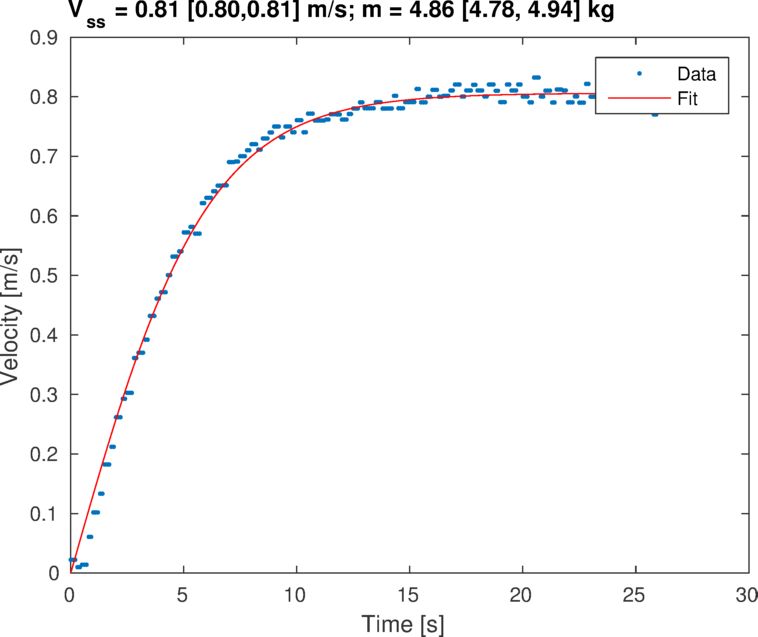
\includegraphics[width=0.9\linewidth]{fit_2.png}
\caption{Results from curve fit.  Parameter values are given as final value and 9\% confidence bounds.}
\label{f:t-cmd}
\end{figure}

\end{document}


